\documentclass[pdftex,ptm,12pt,a4paper]{report}
\renewcommand{\baselinestretch}{1.5}
\setcounter{secnumdepth}{5}

% PDF search & cut'n'paste
\usepackage{cmap}
\usepackage[table,xcdraw]{xcolor}

% Cyrillic support
\usepackage{mathtext}
\usepackage{amsmath}
\usepackage[T1,T2A]{fontenc}
\DeclareSymbolFont{T2Aletters}{T2A}{cmr}{m}{it}
\usepackage[utf8]{inputenc}
\usepackage{multicol}

\usepackage[bottom=30mm,top=20mm,right=20mm,left=30mm,headsep=0cm,nofoot]{geometry}

\usepackage{calc}
\setlength{\footskip}{\paperheight
  -(1in+\voffset+\topmargin+\headheight+\headsep+\textheight)
  -0.75in}

\usepackage{array}
\newcolumntype{C}[1]{>{\centering\let\newline\\\arraybackslash\hspace{0pt}}m{#1}}

\makeatletter
\renewcommand*{\ps@plain}{%
  \let\@mkboth\@gobbletwo
  \let\@oddhead\@empty
  \def\@oddfoot{%
    \reset@font
    \hfil
    \thepage
    % \hfil % removed for aligning to the right
  }%
  \let\@evenhead\@empty
  \let\@evenfoot\@oddfoot
}
\makeatother
\pagestyle{plain}

\usepackage[pdftex]{graphicx}
\usepackage{caption}
\usepackage{subcaption}
\usepackage[russian,english]{babel}
    \addto{\captionsenglish}{\renewcommand{\bibname}{Литература}}
    \addto\captionsenglish{\renewcommand{\figurename}{Рис.}}
    \addto\captionsenglish{\renewcommand{\contentsname}{Содержание}}
    \addto\captionsenglish{\renewcommand{\proofname}{Доказательство}}
\usepackage{hyperref}
\usepackage{url}
\usepackage{abstract}
\usepackage{float}
\usepackage{amsthm}
\usepackage{amssymb}
\usepackage{amsmath}
\renewcommand*{\proofname}{Доказательство}
\usepackage{indentfirst}
\usepackage{color}
\usepackage{natbib}
\usepackage{bbm, dsfont}


% Detect whether PDFLaTeX is in use
\usepackage{ifpdf}

% Fix links to floats
\usepackage[all]{hypcap}

\makeatletter
\renewcommand{\@chapapp}{Часть}
\makeatother

% Theorem Styles
\newtheorem{theorem}{Теорема}[chapter]
\newtheorem{lemma}[theorem]{Лемма}
\newtheorem{claim}[theorem]{Теорема}
% Definition Styles
\theoremstyle{definition}
\newtheorem{definition}{Определение}[chapter]
\newtheorem{example}{Пример}[chapter]
% Rule for Title Page
\newcommand{\HRule}{\rule{\linewidth}{0.5mm}}

\begin{document}

\begin{titlepage}
\newpage

\begin{center}
МИНИСТЕРСТВО ОБРАЗОВАНИЯ И НАУКИ РОССИЙСКОЙ ФЕДЕРАЦИИ \\
\vspace{0.5cm}
ГОСУДАРСТВЕННОЕ ОБРАЗОВАТЕЛЬНОЕ УЧРЕЖДЕНИЕ \\*
ВЫСШЕГО ПРОФЕССИОНАЛЬНОГО ОБРАЗОВАНИЯ\\*
"МОСКОВСКИЙ ФИЗИКО-ТЕХНИЧЕСКИЙ ИНСТИТУТ \\*
(ГОСУДАРСТВЕННЫЙ УНИВЕРСИТЕТ)" \\*
\vspace{0.5cm}
ФАКУЛЬТЕТ ИННОВАЦИЙ И ВЫСОКИХ ТЕХНОЛОГИЙ \\*
КАФЕДРА АНАЛИЗА ДАННЫХ \\*
\hrulefill
\end{center}


\vspace{3em}

\begin{center}
\Large Выпускная квалификационная работа по направлению 01.03.02 <<Прикладная математика и информатика>> \linebreak НА ТЕМУ:
\end{center}

\vspace{2.5em}

\begin{center}
\textsc{\large{\textbf{НЕЙРОСЕТЕВЫЕ МОДЕЛИ В ЗАДАЧАХ ИНТЕРПРЕТАЦИИ ДАННЫХ ФМРТ ПРИ АУДИАЛЬНОЙ СТИМУЛЯЦИИ}}}
\end{center}

\vspace{6.5em}

\begin{minipage}{.45\linewidth}
\begin{flushleft}                           
Студентка \\ Научный руководитель к.ф-м.н \\ Зам. зав. кафедрой д.ф-м.н, проф. 
\end{flushleft} 
\end{minipage}
\hfill
\begin{minipage}{.45\linewidth}
\begin{flushright}                                      
Медведева А.Е.\\ Артемов А.В.\\Бунина Е.И.
\end{flushright} 
\end{minipage}

\vspace{\fill}

\begin{center}
МОСКВА, 2017
\end{center}

\end{titlepage}

\tableofcontents

\sloppy

\chapter{Введение}
\section{ФМРТ в измерении активности мозга}

Функциональная магнитно-резонансная томография, или ФМРТ, - это метод измерения активности головного мозга. Он работает путем обнаружения изменений насыщения крови кислородом, а также изменение кровотока, возникающего в ответ на нейронную активность. Когда зона мозга более активна, она потребляет больше кислорода, и чтобы удовлетворить этот растущий спрос, увеличивается приток крови к рабочей области. ФМРТ может быть использована для создания карт активности, показывающих, какие части мозга вовлечены в конкретный психический процесс.

Каждое ФМРТ измерение -- последовательность трехмерных сканов мозга, где каждый скан есть набор значений сигнала на каждом маленьком участке мозга, называемым вокселем и представляющим собой параллелепипед с сторонами порядка нескольких милиметров (см. \ref{fmri_result}).

\begin{figure}[h]
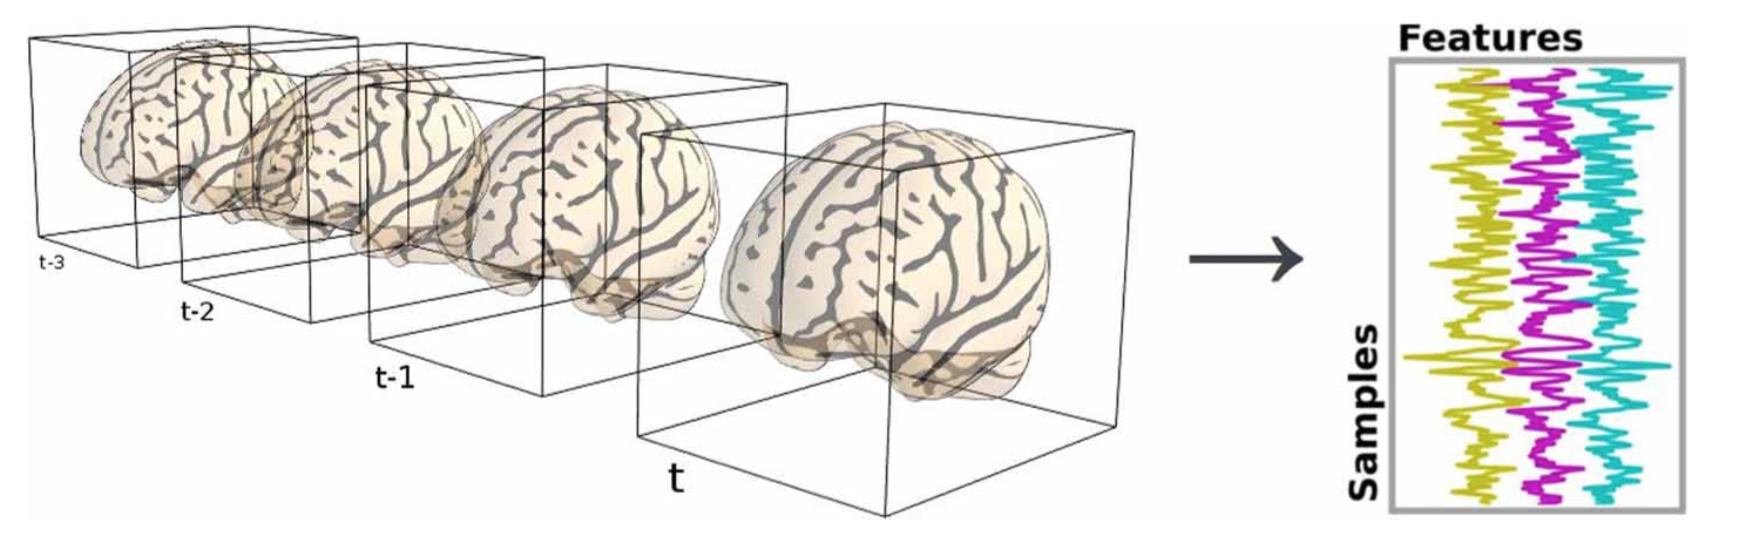
\includegraphics[scale=0.2]{images/fmrt_result.png}
\centering
\caption{ФМРТ измерение.}
\label{fmri_result}
\end{figure}

ФМРТ имеет несколько преимуществ перед другими методами измерения мозговой активности:
\begin{enumerate}
\item Этот метод является неинвазивным и не использует рентгеновское излучение, что делает его безопасным для человека.

\item Имеет хорошую пространственно-временное разрешение. На рисунке \ref{fmri} показано сравнение ФМРТ с другими методами измерения активности мозга, такими как энцефалография(МЭГ, ЭЭГ) и позитронно-эмисионная томография (ПЭТ).

\begin{figure}[h]
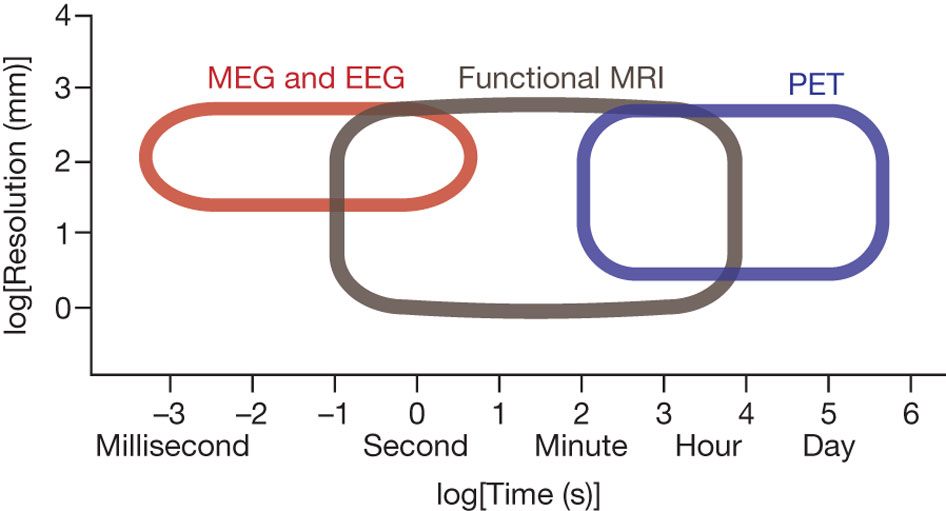
\includegraphics[scale=0.3]{images/fmrt.jpg}
\centering
\caption{Сравнение ФМРТ, ПЭТ и МЭГ.}
\label{fmri}
\end{figure}

\item Его легко использовать для постановки экспериментов и далее анализировать (см. \cite{abraham2014machine}).
\end{enumerate}

Из недостатков можно выделить следующие:

\begin{enumerate}
\item Для точного измерения необходимо, чтобы человек оставался неподвижным. Движения головы, вызванные биением сердца, дыханием и  ерзаньем, являются одним из основных источников шума.

\item Наличие шума, вызванного неоднородностью магнитного поля, используемого для измерения.

\item ФМРТ измеряет уровень активности не напрямую, а косвенно.

\item Уровень насыщения крови кислородом, который измеряет ФМРТ, изменяется очень медленно. Его изменение происходит с некоторой задержкой (обычно порядка пары секунд), так как необходимо некоторое время для реакции сосудистой системы в ответ на потребность мозга в глюкозе. После чего уровень сигнала обычно поднимается до пика примерно через 5 секунд после стимула. Если нейроны остаются активными, пик распространяется на плоское плато. После остановки деятельности, сигнал падает ниже исходного уровня -- явление, называемое недолетом. С течением времени сигнал восстанавливается до базовой линии (см. \ref{hrf}). 

\begin{figure}[h]
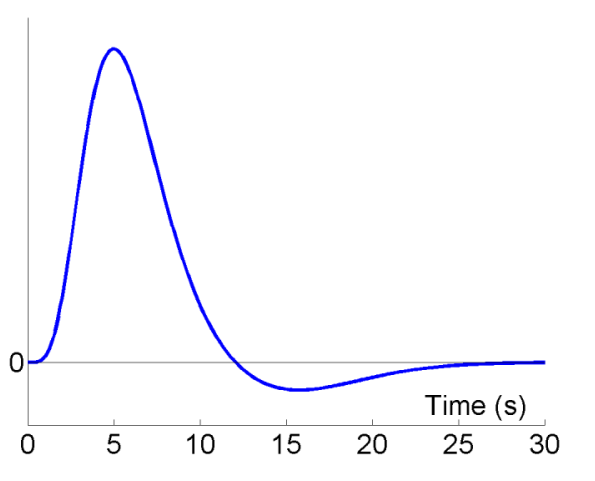
\includegraphics[scale=0.4]{images/hrf.png}
\centering
\caption{Уровень насыщения крови в зависимости от времени.}
\label{hrf}
\end{figure}

\end{enumerate}

\section{Функции зон мозга}

В головном мозге человека ученые выделяют три основные части: задний мозг, средний мозг и передний мозг. Исторически более древними считаются задний и средний мозг. Они отвечают за жизненно важные внутренние функции организма: поддержание тока крови, дыхание. За человеческие формы коммуникации с внешним миром (мышление, память, речь) отвечает передний мозг.

В коре головного мозга можно выделить четыре доли: затылочную, теменную, височную и лобную. В соответствии с принципом латерализации -- разделения по полушариям — каждая доля имеет свою пару (см. \ref{mozg}).

\begin{figure}[h]
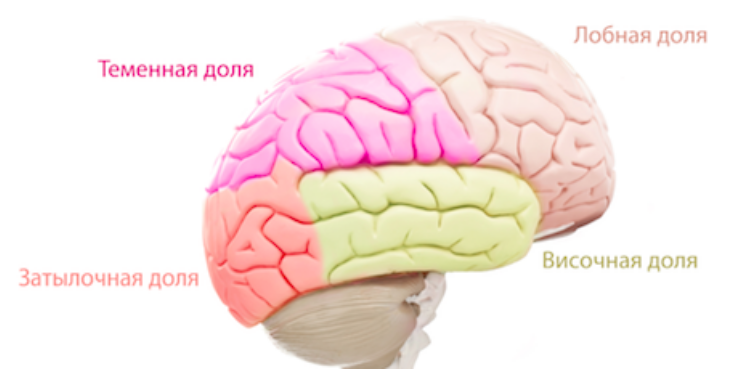
\includegraphics[scale=0.4]{images/mozg.png}
\centering
\caption{Зоны мозга человека.}
\label{mozg}
\end{figure}

Лобные доли можно условно назвать командным пунктом головного мозга. Здесь находятся центры, не столько отвечающие за отдельное действие, сколько обеспечивающие такие качества, как самостоятельность и инициативность человека, его способность к критической самооценке. 
Поражение лобных долей вызывает появление беззаботности, бессмысленных устремлений, переменчивости и склонности к неуместным шуткам. 
С утратой мотивации при атрофии лобных долей человек становится пассивным, теряет интерес к происходящему, часами остается в постели.
Нередко  окружающие принимают такое поведение за леность, 
не подозревая, что изменения в поведении есть прямое следствие гибели 
нервных клеток этой зоны коры головного мозга.

Функции, выполняемые теменными долями, отличаются для доминирующей и недоминирующей сторон. Доминирующая сторона (обычно левая) отвечает за способность понимать устройство целого через соотнесение его частей (их порядок, структуру) и за наше умение складывать части в целое. Это относится к самым разным вещам. Например, для чтения необходимо уметь складывать буквы в слова и слова во фразы. То же с цифрами и числами. Недоминантная сторона (обычно правая) – это центр, который, комбинируя информацию, поступающую из затылочных долей, обеспечивает трехмерное восприятие окружающего мира. Нарушение этой области коры приводит к зрительной агнозии – неспособности распознавать предметы, лица, окружающий пейзаж.

Затылочные доли отвечают за переработку зрительной информации. По сути, все, что мы видим, мы видим не глазами, которые лишь фиксируют раздражение воздействующего на них света и переводят его в электрические импульсы. Мы «видим» затылочными долями, которые интерпретируют поступающие от глаз сигналы. Зная об этом, необходимо отличать у пожилого человека ослабление остроты зрения от проблем, связанных с его способностью воспринимать предметы. Острота зрения (способность видеть мелкие объекты) зависит от работы глаз, восприятие – продукт работы затылочной и теменной долей мозга. Информация о цвете, форме, движении обрабатывается отдельно в затылочной доле коры, прежде чем будет принята в теменной доле для превращения в трехмерное представление. 

Височные доли в верхних отделах обрабатывают слуховые ощущения, превращая их в звуковые образы. Поскольку слух – это канал, по которому человеку передаются звуки речи, височные доли (особенно доминантная левая) играют важнейшую роль в обеспечении речевой коммуникации.
Именно в этой части мозга производится распознавание и наполнение смыслом обращенных к человеку слов, а также подбор единиц языка для выражения собственных смыслов. Недоминантная доля (правая у правшей) участвует в распознавании интонационного рисунка и выражения лица. 
Небольшой участок на внутренней поверхности височных долей, имеющий форму морского конька (гиппокамп), контролируетдолговременную память человека. Именно височные доли хранят наши воспоминания. Доминантная (обычно левая) височная доля имеет дело с вербальной памятью и названиями объектов, недоминантная используется для зрительной памяти.

\chapter{Постановка задачи}

В типичном эксперименте с помощью ФМРТ по внешнему стимулу строится матрица признаков $\textbf{X}.$ Например, при аудиальной стимуляции строки матрицы $\textbf{X}$ -- векторы, соответствующие словам из текста аудио. Измерения ФМРТ -- матрица ответов $\textbf{Y},$ столбцы которой соотвествуют вокселям, строки -- вектор активации мозга в конкретный момент времени. Далее задача сводится к построению модели $f,$ максимизирующую корреляцию Пирсона на тестовой выборке:
$$Pearson(\textbf{Y}_{test},\ f(\textbf{X}_{test})) \rightarrow max_{f}.$$

В случае, если для каждого вокселя своя модель из класса $\mathcal{F}$, то максимизируется средняя корреляция по вокселям. Обозначим число вокселей за $N$, $i$--ый столбец матрицы $\textbf{Y}$ за $\textbf{Y}^{;,i}$. Тогда функционал для максимизации выглядит следующим образом:

$$\frac{1}{N} \sum_{i=1}^{N} Pearson(\textbf{Y}_{test}^{:,i}, f_{i}(\textbf{X}_{test})) \rightarrow max_{\mathcal{F}}.$$

Нетрудно убедится в том, что при нормализованном отклике данная мера эквивалентна минимизации $MSE$. Обозначим $\hat{Y}_i = f_i(\mathbf{X}_{test}), Y = \hat{Y} + \epsilon,$ $\hat{Y}$ независим от $\epsilon$. Учитывая, что $\sigma^2_{Y} = \sigma^2_{\hat{Y}} + \sigma^2_{\epsilon}$, получаем:

$$Pearson(Y, \hat{Y})^2 = \frac{cov^2(Y, \hat{Y})}{\sigma^2_{Y}\sigma^2_{\hat{Y}}} =  \frac{cov(\hat{Y} + \epsilon, \hat{Y})\ cov(\hat{Y} + \epsilon, \hat{Y})}{\sigma^2_{Y}\sigma^2_{\hat{Y}}} = \frac{\sigma^4_{\hat{Y}}}{\sigma^2_{Y}\sigma^2_{\hat{Y}}} = $$

$$= \frac{\sigma^2_{\hat{Y}}}{\sigma^2_{Y}} = \frac{\sigma^2_{Y} - \sigma^2_{\epsilon}}{\sigma^2_{Y}} = 1 - \frac{MSE(Y, \hat{Y})}{\sigma^2_{Y}}.$$

%$$ R^2 = 1 - \frac{\frac{1}{N}\sum_{i=1}^{N} (Y_i - \hat{Y}_i)^2}{\sigma^2_Y} = \frac{\sigma^2_Y - \sigma^2_{\hat{Y}} \frac{1}{N} \sum_{i=1}^{N} (Y_i - \hat{Y}_i)^2}{\sigma^2_Y} = $$

\chapter{Обзор литературы}
\section{Семантический атлас мозга}\label{complex}

\begin{figure}[h]
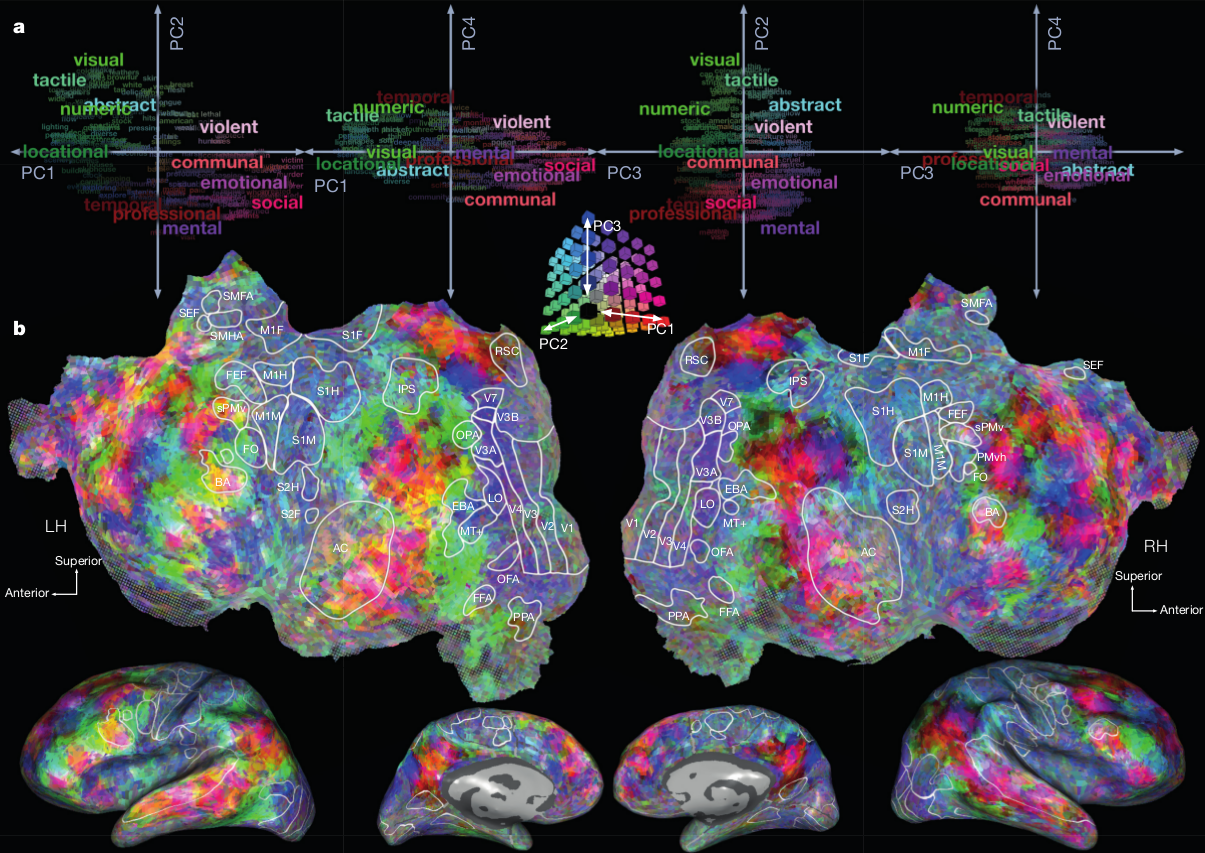
\includegraphics[scale=0.4]{images/galant_results.png}
\centering
\caption{Результаты из работы \cite{huth2016natural}.}
\label{huth_result}
\end{figure}

Работа \cite{huth2016natural} группы американских нейробиологов посвящена созданию семантического атласа мозга на основе данных, полученных с помощью ФМРТ. Ученым удалось выделить области на фронтальной коре, ответственные за конкретные семантические группы, такие как социальные явления, абстрактные понятия, количественные слова. 

\begin{figure}[h]
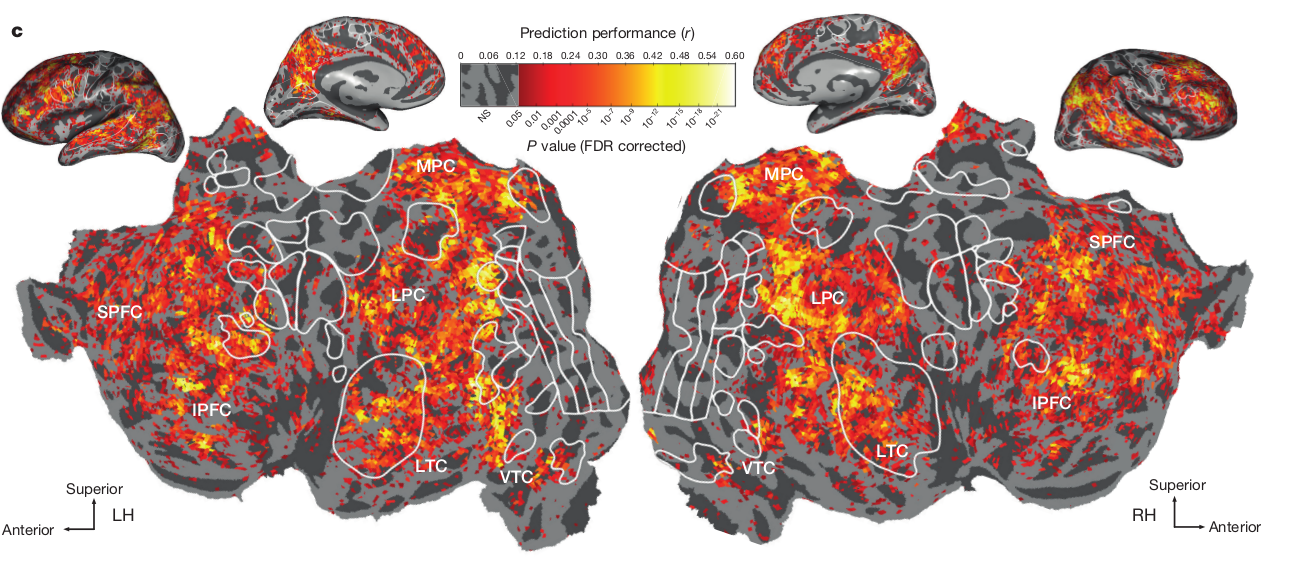
\includegraphics[scale=0.37]{images/map_result_huth.png}
\centering
\caption{Результаты из работы \cite{huth2016natural}.}
\label{map_huth_result}
\end{figure}

Эксперимент был построен следующим образом: 8 испытуемых слушали 2 часа рассказы из радиопередачи. После чего авторы подсчитали на большом корпусе матрицу совместной встречаемости каждого слова из текста аудио и 985 самых часто употребляемых английских слов. Каждая строка этой матрицы соответствовала представлению слова из аудио в 985-мерном пространстве. Для установления зависимости между признаками аудиостимула (представления слов из аудио) и измерениями ФМРТ авторы использовали гребневую регрессию. 
Далее изучались вектора весов регрессии, соответствующей каждому вокселю, для чего они были спроектированы в четырехмерное пространство с помощью метода главных компонент. В это же пространство были спроектированы и слова из аудиостимула. 
С помощью алгоритма k средних спроецированные слова были сгруппированы в 12 категорий. После чего авторы раскрасили пространство из первых трех главных векторов и визуализировали результат (см. \ref{huth_result}). 

Интересна проекция на первую компоненту: положительные знак имеют слова, относящиеся к человеку и человеческим взаимодействиям, отрицательную -- описания восприятия, местоположения, количества. На рис. \ref{map_huth_result} показана средняя корреляция Пирсона в проекции на поверхность долей. Видно, что зоны LTC, VTC, LPC, MPC, SPFC и IPFC предсказываются достаточно хорошо (корреляция значимо больше нуля), ранее эти зоны считались семантической системой мозга.

Также интересно, что височные зоны, отвечающие за анализ слуховой информации, более всего реагируют на слова из социальной группы (см. \ref{gallant_visoc}).

\begin{figure}[h]
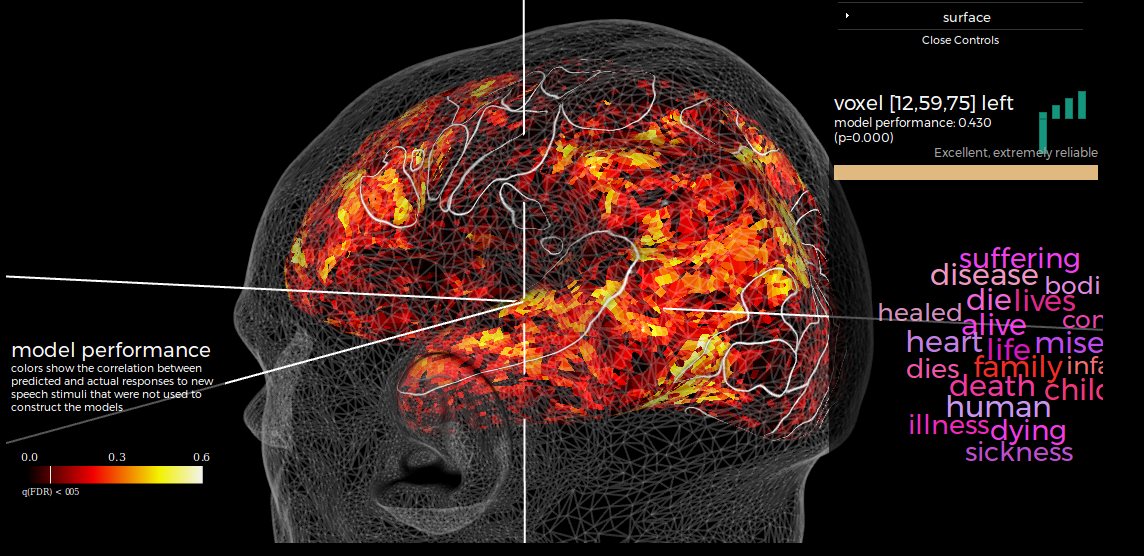
\includegraphics[scale=0.3]{images/gallant_view1.png}
\centering
\caption{Результаты из \cite{huth2016natural}.}
\label{gallant_visoc}
\end{figure}


\section{Применение нейросетевых методов}

\begin{figure}[h]
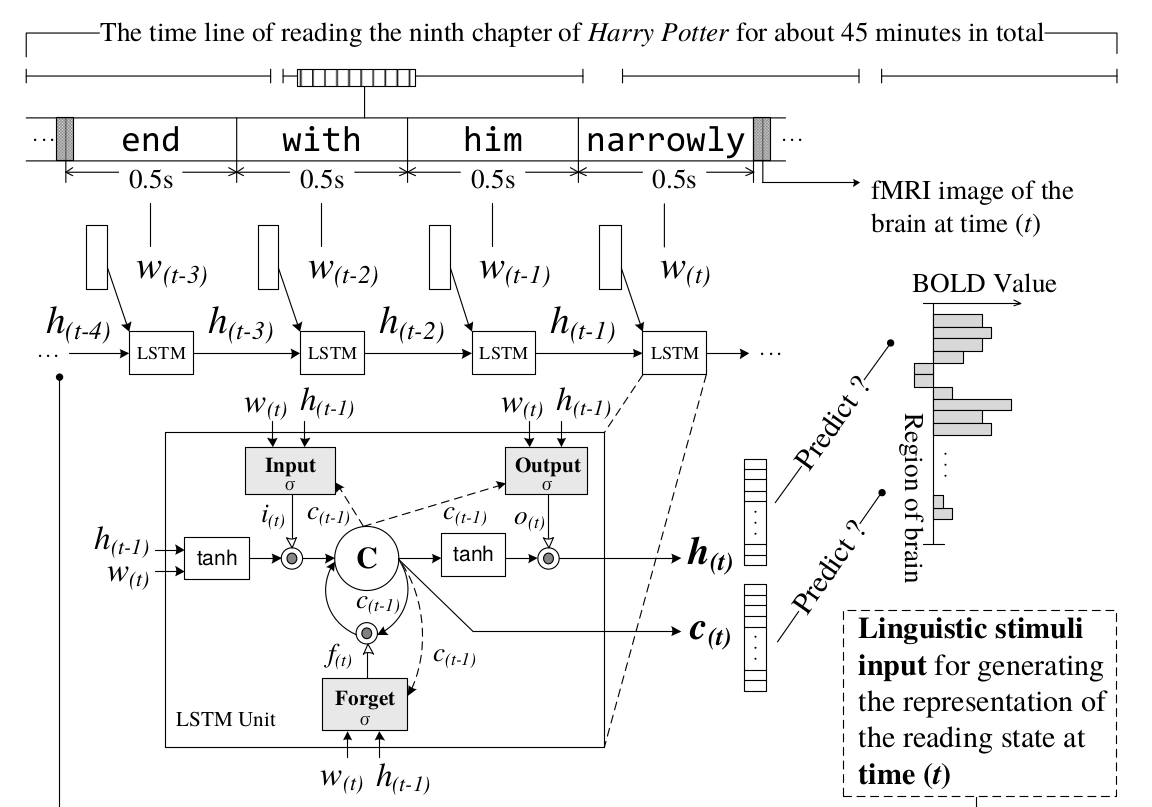
\includegraphics[scale=0.3]{images/lstm.png}
\centering
\caption{Схема эксперимента из \cite{qian2016bridging}.}
\label{ch_experiment}
\end{figure}

В статье \cite{qian2016bridging} изучалось предсказательная способность LSTM юнитов в зависимости от архитектуры (наличия гейтов). Эксперимент был устроен следующим образом: в течение 45 несколько человек равномерно (со скоростью появление слов - 1 слово и полсекунды) читали главу из книги "Гарри Поттер".

Далее авторы обучили на оставшихся главах нейронную сеть, состоящую из одного скрытого слоя  размерности 50, предсказывать следующее слово в тексте. Затем с помощью метода наименьших квадратов устанавливалась зависимость между вектором внутреннего состояния нейросети $a_t$ в момент предсказывания следующего слова и вектором активации всего мозга перед прочтением этого слова (см \ref{ch_experiment}):
$$ y_t = M a_t, a_t \in \{c_t, h_t\}.$$
В качестве вектора внутреннего состояния сети $a_t$ может служить как вектор памяти lstm юнитов $c_t$, так в "внешнее" внутреннее состояние $h_t$ - те значения, которые рекуррентный слой передает полносвязному.
Мерой качества модели авторы использовали косинусное расстояние между предсказанием и действительной активацией мозга, нормализованным на отрезок [0,1]. Несмотря на то, что статья была посвящена изучению LSTM юнитов, авторы получили неплохую предсказательную способность (см. \ref{qian_res}), максимальное качество 0.86 достигалось при максимально возможном окне просмотра на тесте и использовании вектора внутренней памяти сети.

\begin{figure}[h]
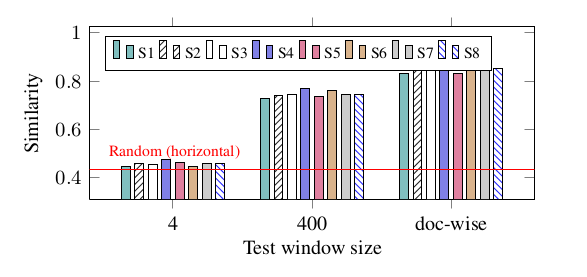
\includegraphics[scale=0.7]{images/neural_nets.png}
\centering
\caption{Результаты из работы \cite{qian2016bridging}.}
\label{qian_res}
\end{figure}

\chapter{Эксперимент}

\section{Описание данных}

Данные были взяты с открытой базы данных ФМРТ openfmri.org (см. \citep{hanke2014high}). В ходе эксперимента 20 носителей немецкого языка в возрасте от 21 до 38 лет 2 часа (8 сегментов по 15 минут) слушали немецкий аудиофильм "Форрест Гамп", версия для слабовидящих. Данная версия отличается от обычной тем, что в моменты, когда нет диалогов, голос за кадром описывает, что происходит на экране. При этом ФМРТ сканер измерял каждые две секунды мозговую активность с пространственным разрешением $2.75\ mm^3$.

\section{Препроцессинг данных}

К данным ФМРТ была применена коррекция движений а также подавление шума с помощью библиотеки FLIRT, затем ФМРТ сигнал был посегментно нормализан, чтобы иметь среднее ноль и дисперсию 1. 

\begin{figure}[h]
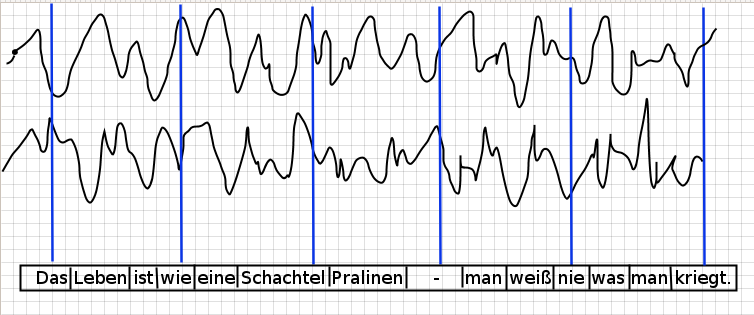
\includegraphics[scale=0.5]{images/word_forrest.png}
\centering
\caption{Визуализация эксперимента.}
\label{interpolation}
\end{figure}

Для дальнейшего работы необходимо знать точное соответствие каждого слова из транскрипции аудио и момента его произношения (выравнивание транскрипции). Так как транскрипция отсутствовала, она создавалась самостоятельно. Сначала на основе описания сцен и субтитров создавалась фразовая транскрипция аудио. Далее каждая фраза и соответствующий фрагмент аудио подавалась на вход библиотеке aeneas, которая выдавала для каждого слова из фразы соответствующий ему момент в аудио. Также был испробован инструмент Google Api Speech Recognition для того чтобы создать более точную версию субтитров, однако данный подход оказался несколько хуже ввиду ошибок распознавания. 

Далее с помощью предобученной модели word to vec слова из транскрипции были переведены в трехсотмерные вектора из $\mathbb{R}^{300}.$ Затем полученные представления слов интерполировались с ядром Ланшица, чтобы согласовать моменты произношения слов и моменты измерения ФМРТ (см. \ref{interpolation}). Ввиду того что отклик конкретного вокселя происходит с некоторой задержкой, а также ввиду сложной формы сигнала отклика (\ref{hrf}), для каждого момента измерения стимул, соответствующий этому моменту, был сконкатенирован с тремя предыдущими (см. \ref{schema}). Таким образом получилось 1200 семантических признаков. Далее из 3600 пар стимул - измерение первые 3100 использовались для обучения и последние 500 для валидации.

\begin{figure}[h]
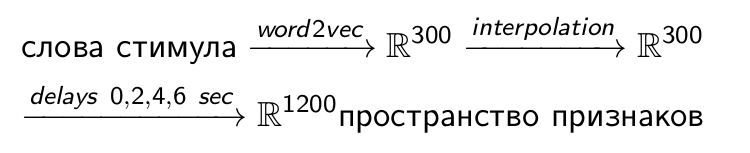
\includegraphics[scale=0.4]{images/schema.png}
\centering
\caption{Схема построения пространства признаков.}
\label{schema}
\end{figure}

\section{Линейные методы}

Повторяя эксперимент авторов статьи \citep{huth2016natural} а также изюегая переобучения, мы использовали повоксельно гребнеую регрессию для предсказания ФМРТ отклика.

\begin{figure}[h]
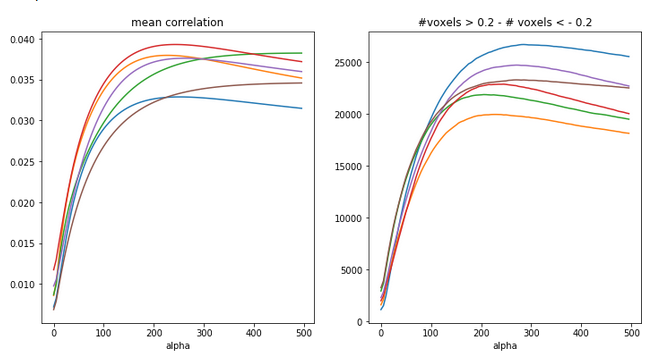
\includegraphics[scale=0.5]{graphics/correlations2.png}
\centering
\caption{Корреляция на тесте в зависимости от параметра $\alpha$ }
\label{corr_many}
\end{figure}

На рисунке \ref{corr_many} показаны результататы корреляции на тесте в зависимости от параметра регулязации альфа гребневой регрессии для 6 человек. На первом графике показана средняя повоксельная корреляция, на втором -- разница числа вокселей, корреляция которых больше 0.2 и числа вокселей, корреляция которых меньше -0.2.

\begin{figure}[h]
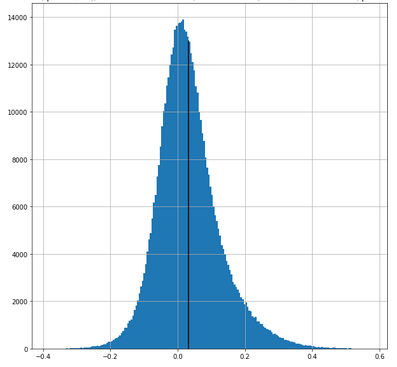
\includegraphics[scale=0.6]{graphics/sub3_prep2.png}
\centering
\caption{Гистограмма корреляций при $\alpha=245$.}
\label{sub3_hist}
\end{figure}

По графику видно, что оптимальные значения параметра альфа примерно одного порядка и средняя корреляция стабильно больше нуля. На рисунке \ref{sub3_hist} показана гистограмма корреляций вокселей для третьего испытуемого.

\begin{figure}[h]
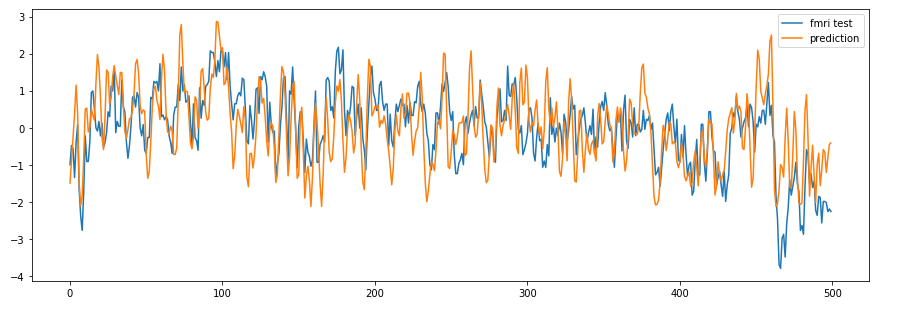
\includegraphics[scale=0.5]{graphics/sub3_prep2_bestvoxel.png}
\centering
\caption{Отклик вокселя и его предсказание.}
\label{sub3_bv}
\end{figure}

\begin{figure}[h]
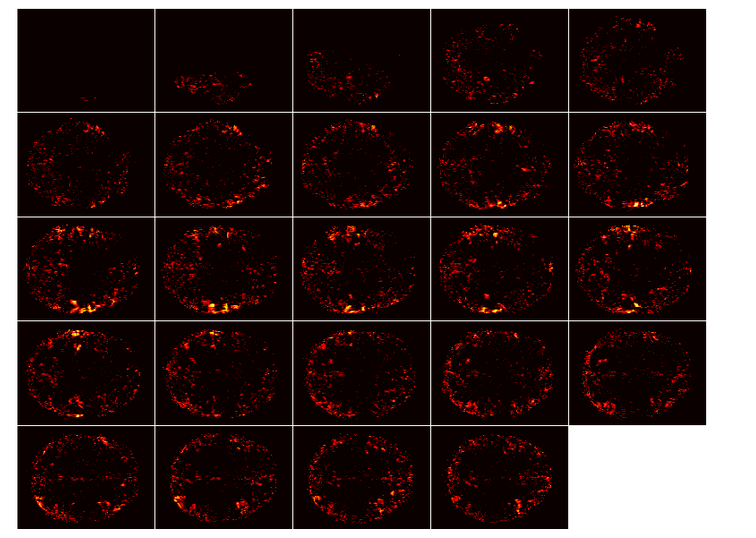
\includegraphics[scale=0.65]{graphics/sub12_trunk01.png}
%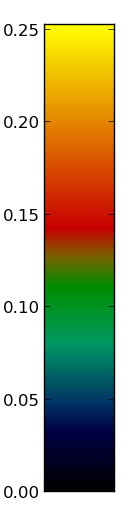
\includegraphics[scale=0.4]{images/colorbar.png}
\centering
\caption{Значимые результаты предсказания (корреляция > 0.1) для 12-ого субъекта.}
\label{sub12_mosaic}
\end{figure}

\begin{figure}[h]
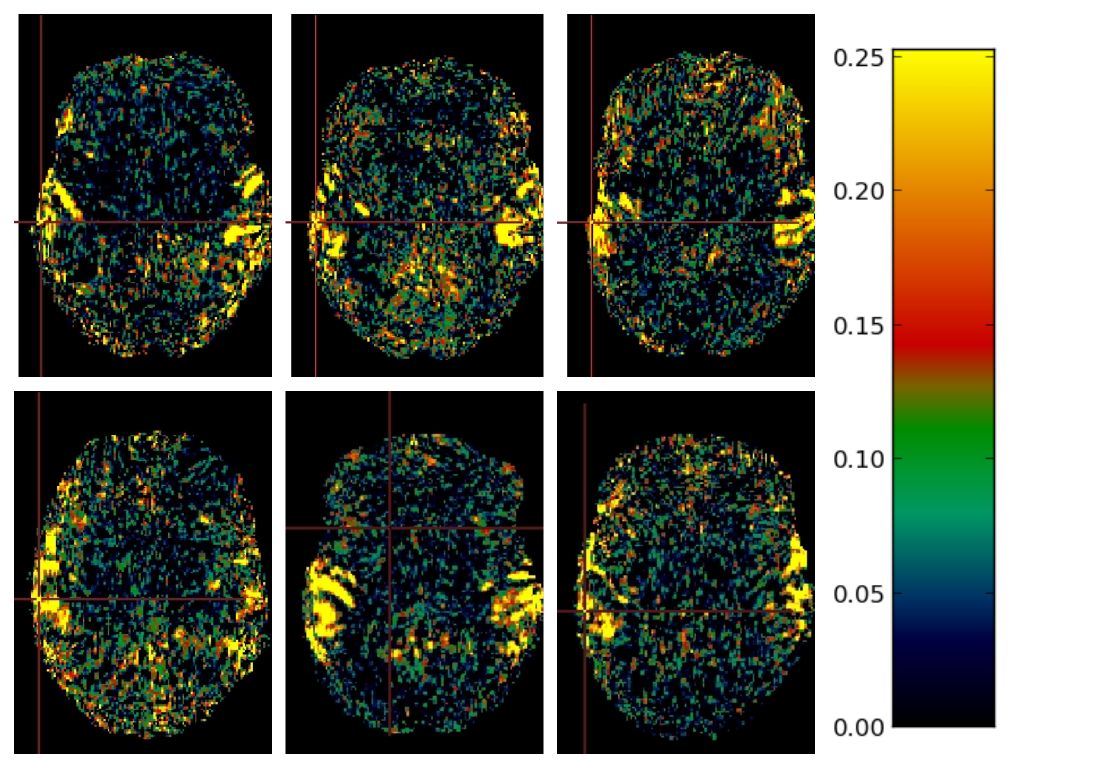
\includegraphics[scale=0.4]{images/all_6.png}
\centering
\caption{Карта корреляции ФМРТ отклика и предсказания.}
\label{slices}
\end{figure}

\begin{figure}
\centering
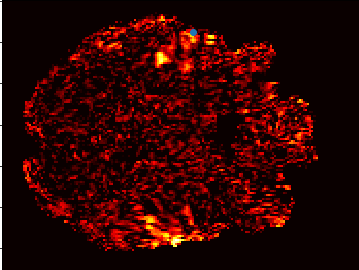
\includegraphics[scale=0.5]{images/voxel_to_choose1.png} 
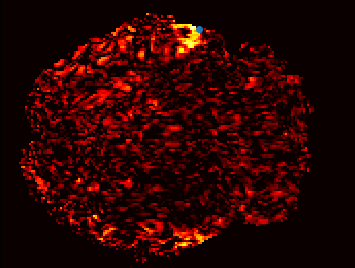
\includegraphics[scale=0.5]{images/voxel_to_choose2.png} 
\caption{Анализ вокселей для двух человек в одной и той же зоне.}
\label{voxel_to_choose}
\end{figure}

\begin{figure}
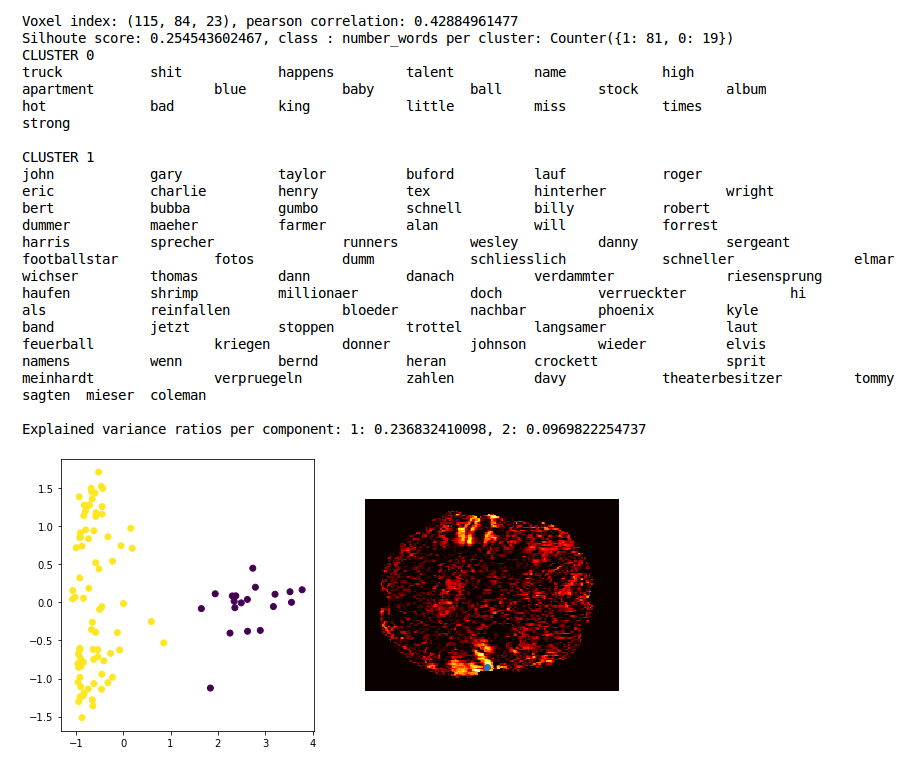
\includegraphics[scale=0.55]{images/sub9_names.png}
\caption{Кластеризация топ 100 слов}
\label{sub9_names}
\end{figure}

\begin{figure}[h]
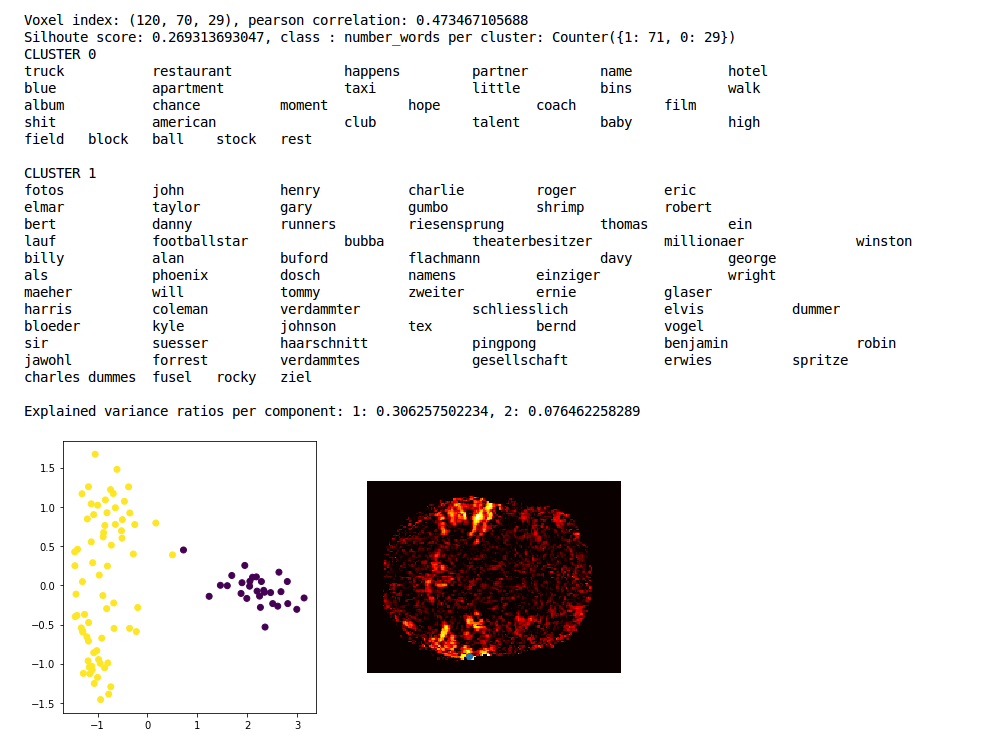
\includegraphics[scale=0.55]{images/sub15_names.png}
\caption{Кластеризация топ 100 слов.}
\label{sub15_names}
\end{figure}
 
Видно, что положительных значений больше и среднее значимо отличается от нуля. 
Критерии согласия Колмогорова для проверки на нормальность показывает p-value равным 0, что означает что данное распределение нельзя считать нормальным. 
Также критерий Вилконсона для проверки на симметричность относительно нуля также дает p-value равным 0.

На рисунке \ref{sub3_bv} показан типичный сигнал ФМРТ и его предсказание, нормализованные для наглядности. Выведем срезы мозга  по оси z -- видим, что хорошо предсказывается височные доли (корреляция достигает 0.4 для всех субъектов), которые отвечают за слух и ассоциативное мышление. 
На рисунке\ref{slices} показаны срезы для этих зон для шести субъектов. Видно, что зоны активации приблизительно повторяют друг друга, на рисунке \ref{huth_result} эти зоны больше всего реагируют на слова из социальной группы. 


\subsection{Анализ весов гребневой регрессии}
После применения гребневой регрессии для каждого вокселя получилось 1200 весов $\vec{v}_{old} \in \mathbb{R}^{1200}$. Эти веса были обратно усреднены по представлениям таким образом, чтобы получить 300 мерные вектора:
$$\vec{w} = \frac{1}{4}\ [(v_1, \ldots, v_{300})^{T} + (v_{301}, \ldots, v_{600})^{T} + (v_{601}, \ldots, v_{900})^{T} + (v_{901}, \ldots, v_{1200})^{T}].$$
Далее для хорошо предсказываемых вокселей искались слова из аудиостимула, косинусное расстояние между представлением которых максимально с данным вокселем.

Интересно, например, что если брать два вокселя в одной у той же зоне у двух человек, и сравнивать топ 20 слов, то у многих зон есть ненулевое пересечение. Например для зоны на рисунке (\ref{voxel_to_choose}) следующее  пересечение:

\begin{itemize}
\item wirklich - собственно, в сущности, на самом деле
\item eigentlich - действительно, в самом деле, право
\item ja - да, конечно, обязательно
\item jawohl -  да, конечно, совершенно верно
\item aber - однако, только, же
\item solltest - должен, быть должным, быть обязанным, следовать, надлежать
\item tust - делать, творить, учинить
\item wirst - становиться, стать, делаться, превращаться
\end{itemize}

Можно выделить слова, со смыслом "действительно", а также глаголы. Продолжая анализировать поучившиеся веса, мы попробовали кластеризовать слова в топе наиболее хорошо предсказываемых вокселей. Часть слов кластеризуется достаточно хорошо: см \ref{sub9_names}, \ref{sub15_names}. На рисунках в нулевом кластере достаточно простые слова: ball, name, miss, high, hot, strong, в первом же много собственных имен: Elvis, Tommy, Danny, Roger. Также точками показана проекция на плоскость с помощью принципа главных компонент, две компоненты объясняют более трети дисперсии, что достаточно много для трехсотмерного представления.

Мы создали демо, в котором можно выбрать человека и воксель, и будет показано на какие слова данный воксель имеет наибольший отклик.

\section{Нейросетевые методы}

\begin{figure}[h]
\centering
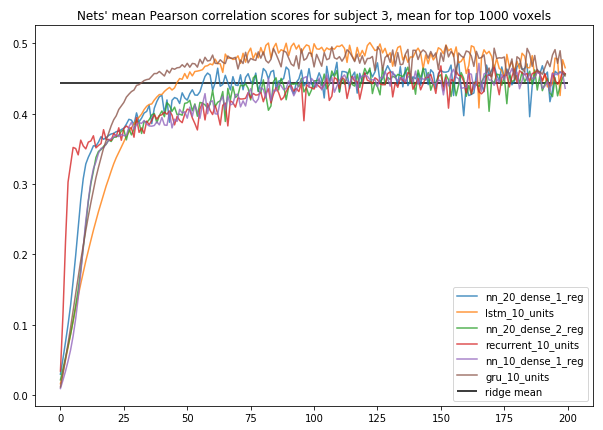
\includegraphics[scale=0.5]{graphics/sub3_net.png}
\caption{Результат на тесте в зависимости от архитектуры сети и эпохи обучения.}
\label{nets_scores}
\end{figure}

В первом приближении мы испробовали предсказывать отклик напрямую на основе синтерполированного представления аудиостимула. На графике \ref{nets_scores} показана средняя корреляция Пирсона на тесте в зависимости от эпохи обучения для 1000 наиболее хорошо предсказываемых по результатам гребневой регрессии вокселей. Горизонтальной линией показан результат гребневой регрессии. Видно, что все архитектуры ведут себя не хуже регрессии, при этом лучший результат у рекуррентной сети (1 скрытый слой с 10 gru/lstm). Это можно объяснить тем, что рекуррентные сети лучше улавливают предыдущий контекст, нежели обычные полносвязные сети.

Так как данных не очень много для того чтобы обучить более мощную модель, мы испробовали несколько другой подход. 
Мы обучили нейронную сеть (см. \ref{lstm_architecture}) с одним скрытым LSTM слоем размерности 50 и трехсотмерным представлением, проинициализированным предобученным word2vecом, использовавшемся в гребневой регрессии, предсказывать следующее слово на корпусе, состоящем из 13 немецких книг и 200000 статей немецкой википедии. Статьи википедии выбирались таким образом, чтобы треть хотя бы одна треть слов из статьи присутствовала в аудиостимуле.

\begin{figure}
\centering
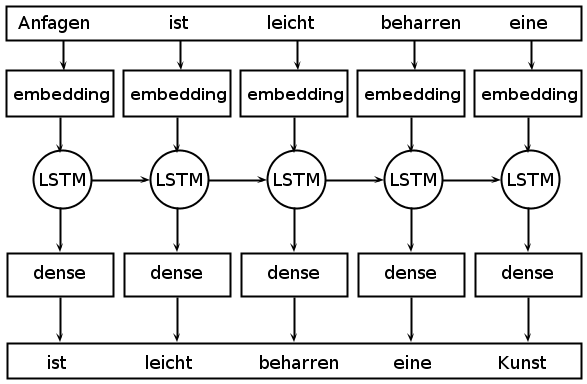
\includegraphics[scale=0.5]{images/lstm-architecture.png}
\caption{Работа сети на примере фразы: Anfagen ist leicht, beharren eine Kunst.}
\label{lstm_architecture}
\end{figure}

Далее через эту сеть был пропущен аудиостимул и каждому слову сопоставлялось состояние lstm слоя в момент предсказания следующего слова. Далее новые полученные представления также интерполировались и конкатенировались и на основе их предсказывался отклик 1000 наиболее хорошо предсказываемых вокселей по результатам гребневой регрессии.
Оказалось, что данное представление дает результат не хуже гребневой регрессии, при этом использует пятидесятимерное семантическое  пространство, а не трехсотмерное.

\section{Избирательность в нейросетевых подходах}
\begin{figure}
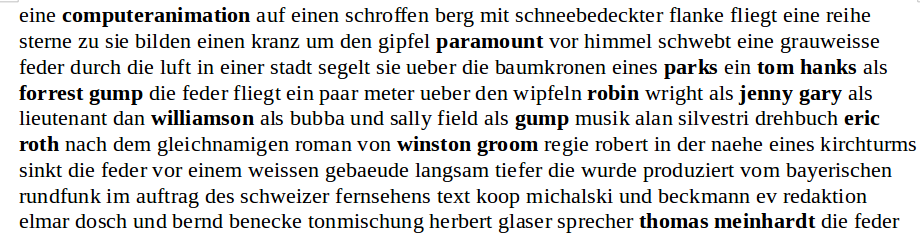
\includegraphics[scale=0.5]{images/text_crop_wb.png}
\caption{Активации рекуррентного нейрона на слова аудиостимула. Наибольшие активации выделены жирным шрифтом.}
\label{lstm_activation}
\end{figure}

Далее мы попробовали проинтерпретировать веса гребневой регрессии. Для этого мы рассмотрели тот lstm unit, вес которого по модулю наибольший и посмотрели его активации на слова из аудиостимула. Оказалось, что наибольшая активациия достигается на собственный именах (см \ref{lstm_activation}).

\chapter{Сравнение моделей}

\chapter{Заключение}

\bibliography{diplomnaya_rabota}
\bibliographystyle{plain}

\end{document}














